\begin{center}
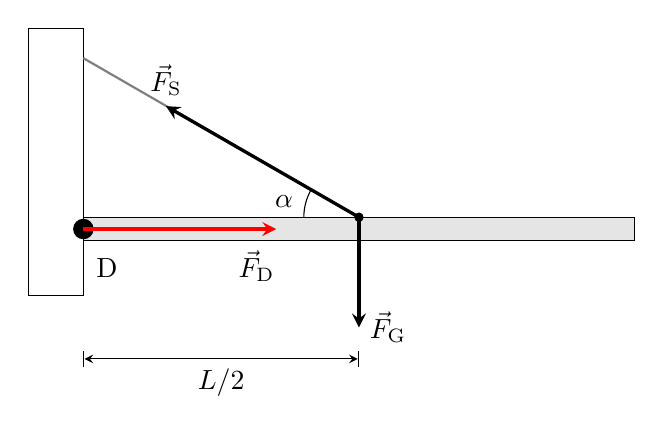
\begin{tikzpicture}[>=stealth]
 \draw (-0.7,-1.0) rectangle (0,2.4);
 \fill[gray!20] (0,-0.3) rectangle (7,0);
 \draw (0,-0.3) rectangle (7,0);
 \draw[thick, gray] (0,2.02) -- (3.5,0);
 \fill (0,-0.15) circle (0.13);
 \node at (0.3,-0.65) {D};
 \fill (3.5,0) circle (0.06);
 \draw (2.8,0) arc (180:150:0.7);
 \node at (2.55,0.2) {$\alpha$};
 \draw[->, very thick] (3.5,0) -- (1.05,1.41) node[above] {$\vec F_\mathrm{S}$};
 \draw[->, very thick] (3.5,0) -- (3.5,-1.4) node[right] {$\vec F_\mathrm{G}$};
 \draw[->, very thick, red] (0,-0.15) -- (2.45,-0.15);
 \node[below] at (2.2,-0.3) {$\vec F_\mathrm{D}$};
 \draw[|<->|] (0,-1.8) -- (3.5,-1.8) node[midway, below] {$L/2$};
\end{tikzpicture}
\end{center}

Auf die Brücke wirken die Gewichtskraft $F_\mathrm{G} = m\,g$ im Schwerpunkt (Mitte), die Seilkraft $F_\mathrm{S}$ in der Mitte und die Kraft $\vec F_\mathrm{D}$ im Drehpunkt. Das Seil schliesst mit der Brücke den Winkel $\alpha$ ein; senkrecht zur Brücke wirkt die Komponente $F_\mathrm{S}\sin\alpha$.

Das Drehmoment von $\vec F_\mathrm{D}$ um D ist null. Gleichgewicht der Drehmomente um D (beide übrigen Kräfte greifen im Abstand $L/2$ an):
\begin{align}
 F_\mathrm{S}\sin\alpha\cdot\frac{L}{2} &= m\,g\cdot\frac{L}{2}
\end{align}
Mit $m\,g = \FGzF = \mZb\cdot\gE = \FGz$ folgt
\begin{align}
 \alpha &= \alZF = \arcsin\left(\frac{\FGz}{\FSz}\right) = \alZ \approx \result{\alZP{0}{2}}
\end{align}
Kräftegleichgewicht: Senkrecht hebt die Seilkraftkomponente $F_\mathrm{S}\sin\alpha = m\,g$ die Gewichtskraft bereits auf, die Kraft im Drehpunkt hat also keine senkrechte Komponente. Waagrecht muss sie die Komponente $F_\mathrm{S}\cos\alpha$ des Seils (zur Wand hin) ausgleichen:
\begin{align}
 F_\mathrm{D} &= F_\mathrm{S}\cos\alpha = \FDzF \\
   &= \sqrt{\left(\FSz\right)^2-\left(\FGz\right)^2} \\
   &= \FDz \approx \result{\FDzP{3}{2}}
\end{align}
Die Kraft im Drehpunkt zeigt waagrecht von der Wand weg (in der Skizze nach rechts): Das Lager drückt die Brücke von der Wand weg, weil das Seil sie zur Wand hin zieht.
